
%%% Local Variables: 
%%% mode: latex
%%% TeX-master: t
%%% End: 


\documentclass{sig-alternate}

% Housekeeping
% Proudly writing in Emacs with TeXLive 2012 under Debian 7.3.
\usepackage{amsmath}
\usepackage{amssymb}

\usepackage{cite}
\usepackage{algorithmic}
\usepackage{array}
\usepackage{graphicx}
\graphicspath{{./}{./Figure/}}

\usepackage{url}





% This should be put last.
\usepackage{hyperref}





\begin{document}
\title{Improving Building Energy Efficiency by Kinect-based Occupancy
  Tracking and Mobility Detecting System}

  
\numberofauthors{1} 
\author{\alignauthor Haleimah Al Zeyoudi, Yanan Xiao, Chi-Kin Chau \\
  \quad \\  
\affaddr{Masdar Institute of Science and Technology} \\
\affaddr{ \{hzeyoudi, yxiao, ckchau\}@masdar.ac.ae}
} 



\makeatletter
\let\@copyrightspace\relax
\makeatother



% \numberofauthors{1}
% \author{
% \alignauthor
% Some author
% }


\maketitle{}



\begin{abstract}
 Nowadays, most building air conditioning systems often operate on a
 fixed schedule rather than based on real-time occupancy. In this
 paper, we develop an occupancy tracking software based on MS Kinect
 to capture the number of people in an open lab. We then employ a
 Markov Chain (MC) model for its occupancy transitions. We apply our
 occupancy model to simulate a dynamic HVAC schedule on eQuest, and
 obtain up to 22.1\% energy reduction in HVAC.  
\end{abstract}

% I comment out this part. It seems that it's useless.

% \category{C.3}{Special-purpose and application-based
%   systems}{Real-time and embedded systems}

% \terms{Algorithms, Design, Management}

% \keywords{Wireless sensor networks, Markov chain, Simulation}





% What the heck am I reading.


\section{Introduction}
\label{sec:introduction}
The majority of energy consumption in modern buildings is due to
Heating Ventilation and Air Conditioning (HVAC) systems, which are
often designed to operate at full capacity most of the time and it is
often assumed a maximum occupancy~\cite{ref:Wang2011}. Although the
current HVAC systems are equipped with presence sensors, their
sensitivity is problematic for management and control systems, and
cannot accurately capture the dynamic occupancy patterns in
buildings. In addition, they are unable to proactively adjust to
occupants' comfort levels. Understanding human mobility and occupancy
patterns is a key factor in order to successfully manage HVAC systems
in buildings. The main contribution of our paper is to develop an
energy-saving system based on accurate occupancy patterns of human
mobility in buildings. The most important features of the system are
as follows: a) A real-time detection and tracking of human mobility in
buildings based on Kinect. b) An occupancy prediction mechanism using
Markov chain model. % This part should be concised.  
\par






\section{Implementation}
\label{sec:implementation}

\subsection{Kinect-based Occupancy Counting Software}

Our occupancy counting software is developed using Microsoft Visual
C\# 2010, project WPF application in C\# and XML\@. Both types of
Kinect are used and tested to insure that it works properly, i.e. Xbox
Kinect and Kinect for Windows.    
\par
% In the next paragraph I would sum up the functions of this software
% and some extras behind it.

Kinect can capture RGB and depth images with the help of color sensor
as well as infrared (IR) sensor. The depth image as shown in
Figure~\ref{fig:system-arch}. For each depth image captured, a
corresponding blue box with unique ID is drawn to detect the movement
of multiple people at the same time. We implemented a system that can
count occupancy based on head tracking and skeletal tracking with a
high accuracy.  


\subsection{Testbed Setup}
\label{sec:testbed-setup}

The testbed environment in our experiment is an open laboratory with
no walls. Therefore we divide this lab into 4 zones and deployed 8
Kinect sensors attached to a laptop running Windows at key areas of
each zone, i.e.\ the conceptual entrance and exit. The image of In/Out
is captured by Kinect and processed by our system to track
mobility. All mobility data is recorded by offline processing. A
selection of deployments is shown in
Figure~\ref{fig:kinect-deployment}.  




\begin{figure}[!tb]
  \centering
  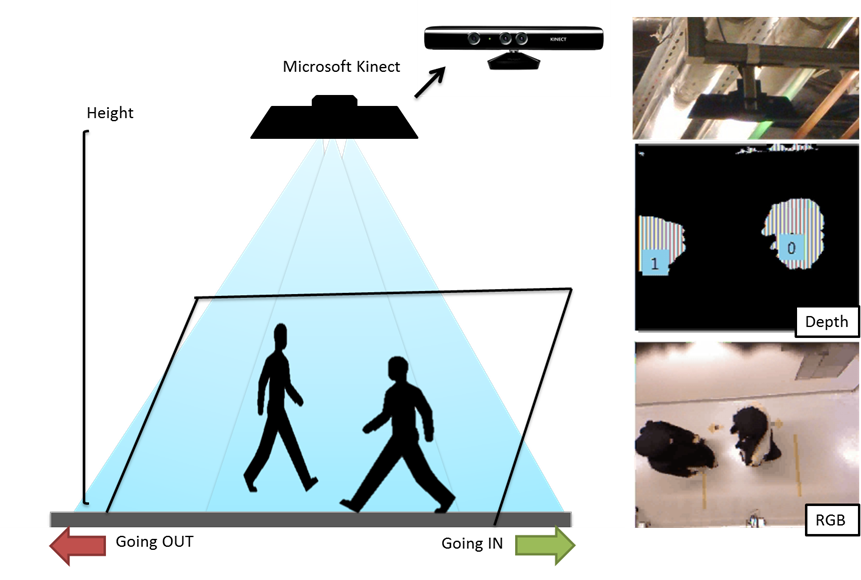
\includegraphics[scale=0.6]{minisys}
  \caption{Architecture of human mobility tracking system}
  \label{fig:system-arch}
\end{figure}

\begin{figure}[!tb]
  \centering
  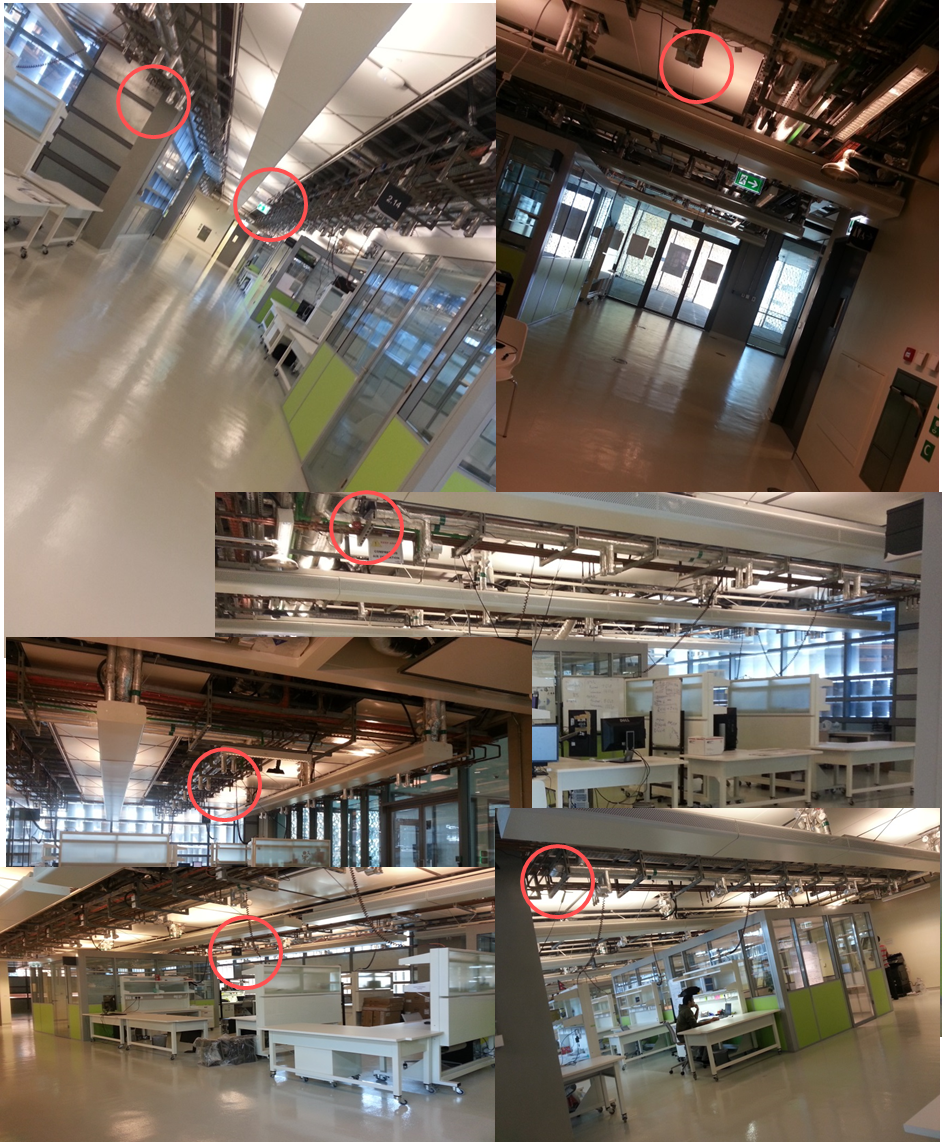
\includegraphics[scale=0.5]{realworld}
  \caption{Kinect deployments in an open lab}
  \label{fig:kinect-deployment}
\end{figure}



\subsection{Markov Chain Prediction Model}
\label{sec:mark-chain-pred}

% Life is never easy. Especially when you are a graduate student.

We employ a Markov chain model for a prediction model of mobility
across different zones, which is built on the work
in~\cite{ref:Erickson:2009,ref:Erickson:2010}. We parse mobility data
and fit the distribution of occupancy data, i.e.\ number of people at
a specific time slot in each zone. We use a time slot as 30min and
divide the states of occupancy into 4 occupancy states: E for empty, F
for few, M for medium and C for crowded. For each time slot, an
occupancy state is assigned with respect to the number of people in
that zone. For example, when the number lies in between 8 and 14, then
the state is assigned to be M.  


\par
% In this part we will describe how the transition matrix is built and
% how it ``seemingly'' works.

To corroborate the accuracy of our Kinect detection system, we compare
the processed occupancy data against the ground truth, which is
collected by manually counting the number of people in captured
videos.  We observe over 90/% accuracy in our Kinect detection system.  

Next, we use the occupancy data to obtain a Markov chain model, which
is a 256-by-256 matrix, representing the joint occupancy states in the
four zones. 


\par
The matrix we obtain is very sparse, because many states has no
transition probability as reflected from real mobility patterns. We
present the Markov chain model in
Figure~\ref{fig:transitional-matrix}. This transition matrix is then
used to enable a dynamic control strategy for ventilation and air
conditioning systems.  



\begin{figure}[!tb]
  \centering
  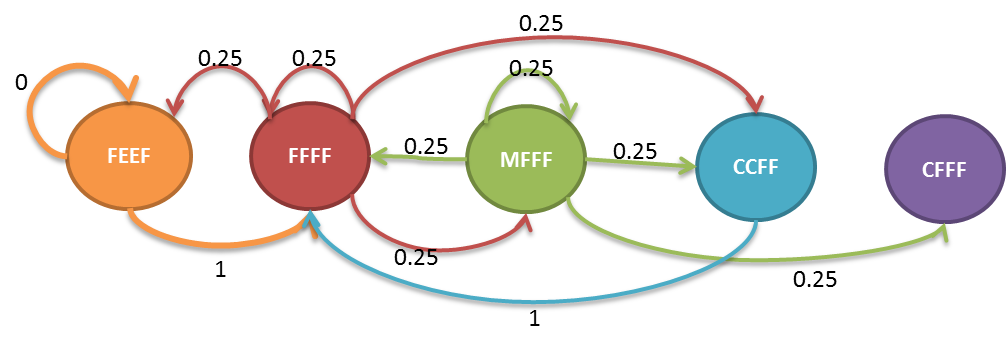
\includegraphics[scale=0.45]{mcc}
  \caption{Transition matrix of occupancy states.}
  \label{fig:transitional-matrix}
\end{figure}


% I am planning whether to add some more stuff about Markov Chain or
% not. Since, well, the OUTLINE of Mrs. Haleimah's thesis is
% unclear. Even if you do not have romance, you should focus on your
% research. 

\section{Simulation}
\label{sec:simulation}

We carry out simulation studies by eQuest by creating a building model
and setting parameters to corresponding our buildings. The model is a
two-floor office building with a total floor area of $232m^{2}$. Each
floor is divided into four office zones with a floor area of $40m^{2}$
each. Windows are placed on the north, east and west walls of the
building with overhangs having a projection factor (overhang
depth/window height) of $0.6$. Two doors are placed on the north and
east sides of the building. Windows and doors are not specified on the
south wall to minimize heat gain through radiation. The window to
gross wall area is kept at 29\%. The cooling system is configured to
match practical office in our office.  



\section{Results}
\label{sec:results}
We adopt two control strategies to investigate their effect by our
model. In the simulation, we use a fixed set-point for air
conditioning system while applying a dynamic occupancy schedule
generated from Markov chain model. We compare the energy consumption
between HVAC schedule set according to the observed average occupancy
with the original HVAC schedule set according a building design guide
that assumes a maximum occupancy throughout the weekdays. We next
apply a more realistic schedule with a dynamic set-point that varies
according to the occupancy states. The more populated a zone is, the
lower set-point it requires. Our simulation result is shown in
Figure~\ref{fig:energy-consumption}. The observed energy saving is up
to 22.1\% in July.  



\begin{figure}[!tb]
  \hspace{-20pt}
  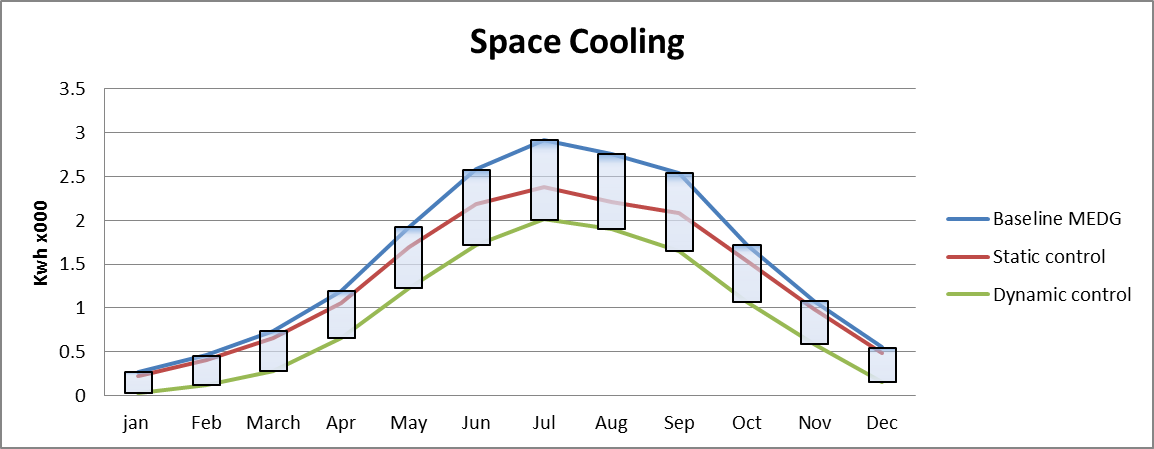
\includegraphics[scale=0.5]{sc}
  \caption{Energy consumption of 3 different control strategies}
  \label{fig:energy-consumption}
\end{figure}




% \section{Related Works}
% \label{sec:related-works}


% Comment: I know till now this project sucks. Well, I am not the
% ``main contributor'' and ...



\section{Conclusion and Future Work}
\label{sec:concl-future-work}

We aim to develop a system to improve the energy efficiency in our
campus by making the building management systems smarter to
dynamically adjust the HVAC system. Currently, we have developed a
Kinect-based mobility tracking system to identify accurate the state
of occupancy in an open lab. We devise a mobility model using Markov
Chain to predict the likelihood of each zone's next occupancy
state. Furthermore, we have conducted simulations to investigate the
energy reduction. We plan to extend our Markov chain model to capture
human activities besides of occupancy.  







\bibliographystyle{plain}
\bibliography{sigproc}


\end{document}


% End of the day
% Successfully ``manage energy'' in buildings. What the heck am I
% reading and writing.
% I have to take part in the next BIG meeting with several
% professors. If possible, I would put forward a plan on HOW TO do
% those smart building buddies.

% Do not rush. Take time and show those reviewers what the heck you
% are doing and to which degree you plan to achieve.